\documentclass{standalone}
\usepackage{tikz}

\begin{document}

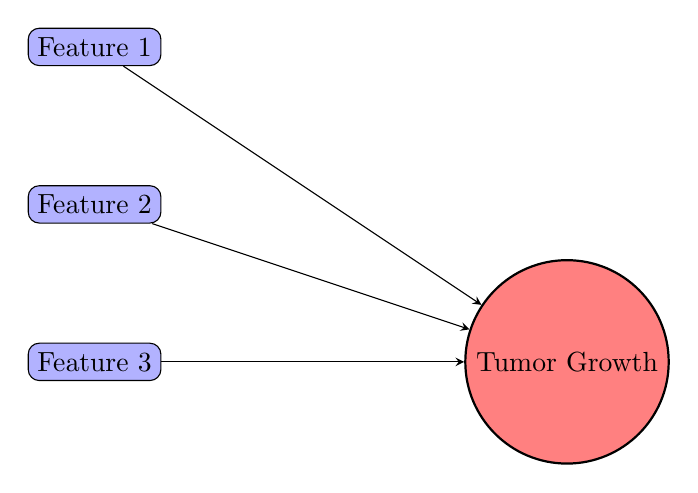
\begin{tikzpicture}[node distance=2cm]
    % Nodes for features X
    \node[draw, fill=blue!30, rounded corners] (X1) {Feature 1};
    \node[draw, fill=blue!30, rounded corners, below of=X1] (X2) {Feature 2};
    \node[draw, fill=blue!30, rounded corners, below of=X2] (X3) {Feature 3};

    % Node for endpoint y (Tumor Growth)
    \node[draw, fill=red!50, circle, thick, right of=X3, xshift=4cm] (y) {Tumor Growth};

    % Arrows to show relationships
    \draw[-stealth] (X1) -- (y);
    \draw[-stealth] (X2) -- (y);
    \draw[-stealth] (X3) -- (y);
\end{tikzpicture}

\end{document}